% Multiple Choice Question 6

\begin{center}
    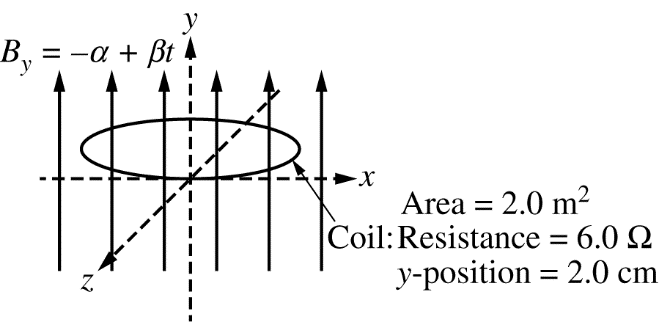
\includegraphics[scale=0.4]{images/img-005-008.png}
\end{center}

\begin{questions}
\setcounter{question}{5}

\question
The $y$-component of the magnetic field $B$ is given as a function of time $t$ by the equation $B_{y}=-\alpha+\beta t$, where $\alpha=4.0 \unit{T}$ and $\beta=3.0 \unit{T/s}$. A coil of wire with an area of $2.0 \unit{m^2}$ and a resistance of $6.0\mathop{\Omega}$ is placed in this field, parallel to the $xz$-plane at $y=2.0 \unit{cm}$. The current in the coil at time $t=1.2 \unit{s}$ is most nearly

\begin{oneparchoices}
    \choice $0$
    \choice $0.6\unit{A}$
    \choice $1.0\unit{A}$
    \choice $3.6\unit{A}$
    \choice $6.0\unit{A}$
\end{oneparchoices}

\end{questions}
